\section{Preparation of a q-sample}
\label{part4}

Given a discrete Bayesian network, it is possible to sample the underlying probability distribution using a quantum circuit. Indeed, this sampling method harnesses the computational advantages offered by quantum algorithms, notably through techniques such as amplitude amplification discussed in previous sections. \cite{borujeni2021quantum}

\subsection{Description}
The construction of the quantum circuit that prepares a state vector representative of the Bayesian network, referred to as a \textit{q-sample}, nvolves three primary steps:
\begin{itemize}
\item[1] Associate each variable of the Bayesian network with one or more qubits (depending on the number of values taken by the variable).
\item[2] Associate the probabilities (marginal or conditional) of each variable with the amplitudes of the component states of the corresponding qubits.
\item[3] Realize the amplitudes of the quantum states using (controlled) rotation gates, in a topological order of the graph $G$.
\end{itemize}
Initially, we shall consider the binary case where the variables of the Bayesian network take only two values.
\\[5pt]
Let $\mathcal{B} = (G,\mathcal{X})$ be a Bayesian network with $G=(V,E)$ a directed acyclic graph and $\mathcal{X}=(X_i)_{i\in[\![1,k]\!]}$ a family of random variables taking values in $\{0,1\}$ defined on $(\Omega, \mathcal{F}, \mathbb{P})$. We define the isomorphism:
\begin{align*}
    \Psi : \mathcal{X} &\longrightarrow \mathbb{C}^2\\
    X_i &\longmapsto |\psi_i\rangle
\end{align*}
which associates each variable of the Bayesian network with a state vector implemented by a qubit of the circuit. Thus, we represent the family $\mathcal{X}$ of random variables by a single state vector using the tensor product:
\[|\psi\rangle = \bigotimes_{i=1}^{k}|\psi_i\rangle \in (\mathbb{C}^2)^{\otimes k}\]
In practice, the vectors $|\psi_i\rangle$\footnotemark \ are initialized to $|0\rangle$ during their initialization in the circuit. We must then assign them the appropriate amplitudes to obtain the probabilities of the random variable upon measurement. In other words, for all $i\in[\![1,k]\!]$, we want to obtain:
\[|\psi_i\rangle = \alpha_i|0\rangle + \beta_i|1\rangle\]
with $|\alpha_i|^2 = \mathbb{P}(X_i=0)$ and $|\beta_i|^2 = \mathbb{P}(X_i=1)$.
\footnotetext{For simplicity, we will use the terms "qubits" and "state vectors" interchangeably and similarly the terms "quantum gates" and "unitary operators".}
\\[5pt]
We distinguish two cases:
\begin{itemize}
\item Variables $X_i$ without parents in $G$: These are treated first. We apply a rotation gate $R_Y$ with an angle $\theta$ to assign the probabilities of a random variable to its representative qubit. The definition of $R_Y$ and the calculation of $\theta$ are explained in subsection \ref{simple_rotation_calc}.
\item Variables $X_i$ with parents in $G$: These are treated second in a topological order of the graph $G$. Moreover, several angles will need to be calculated for the different rotations conditioned by the values taken by the parents of $X_i$. Since the variables are binary, for $|Pa(X_i)|=m_i$, we have $2^{m_i}$ rotations to determine and apply to the vector $|\psi_i\rangle$. These rotations are implemented by controlled rotation gates whose angles depend on the conditional probabilities of $X_i$. Their calculation is detailed in subsection \ref{multi_rotation_calc}.
\end{itemize}

\subsection{Bloch Sphere}
\label{section_Bloch}

\begin{figure}
\centering
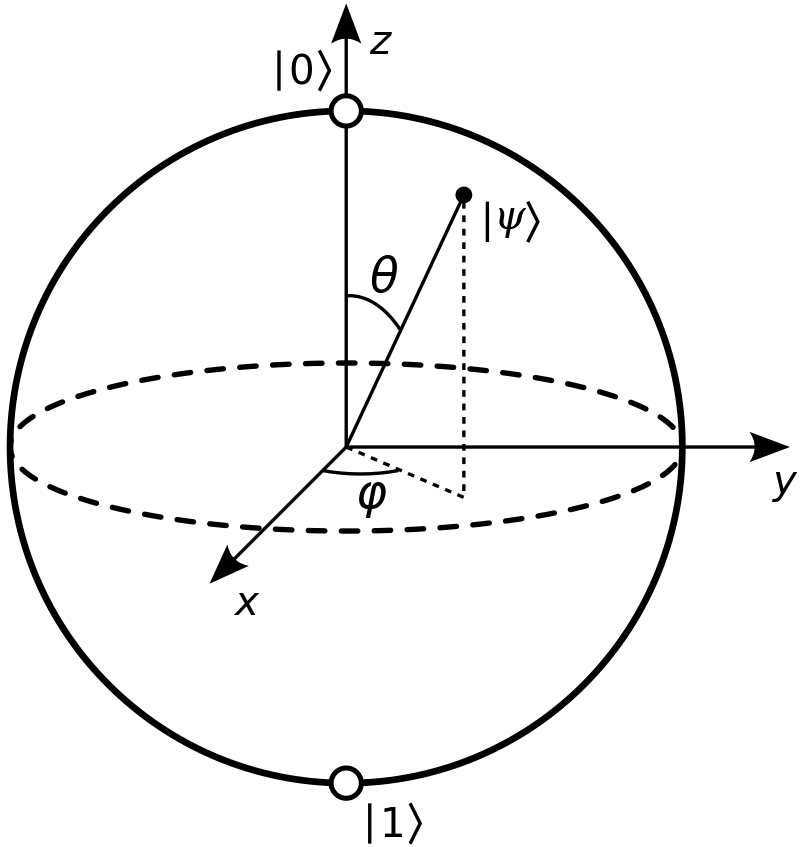
\includegraphics[scale=0.2]{Bloch_sphere}
\caption{The Bloch Sphere}
\label{fig:Bloch}
\end{figure}

To begin, we define the Bloch sphere (Figure \ref{fig:Bloch}) which graphically represents the state space of a single qubit. The Bloch sphere provides an intuitive visualization of how quantum gates transform qubit states. Notably, it includes the rotations induced by the $R_Y$ gate, among others.
\\[5pt]
Consider a state $|\psi \rangle =\alpha |0\rangle +\beta |1\rangle$ with amplitudes $\alpha ,\beta \in \mathbb{C}$. In polar coordinates, there exist $r_{\alpha}, r_{\beta} \in \mathbb{R}_+$ and $\phi_{\alpha}, \phi_{\beta} \in [0,2\pi[$ such that:
\[|\psi \rangle = r_{\alpha}e^{i\phi_{\alpha}}|0\rangle + r_{\beta}e^{i\phi_{\beta}} |1\rangle\]
\\[5pt]
Since $|re^{i\phi}|^2 = re^{i\phi}re^{-i\phi} = r^2$, the probability of observing a qubit is entirely determined by the modulus of its amplitude. We thus define the equivalence relation $\sim$ on $\mathbb{C}^2$ by $\alpha \sim \beta \iff |\alpha|^2=|\beta|^2$. We have:
\[|\psi \rangle \sim r_{\alpha}|0\rangle + r_{\beta}e^{i(\phi_{\beta}-\phi_{\alpha})} |1\rangle\]
Moreover, since $r_{\alpha}^2+r_{\beta}^2=1$ and $r_{\alpha}, r_{\beta} \in [0,1]$, there exists a unique $\theta \in [0,\pi]$ such that $(r_{\alpha}, r_{\beta}) = (\mathrm{cos}(\theta/2),\mathrm{sin}(\theta/2))$. By setting $\phi = \phi_{\beta}-\phi_{\alpha} + 2n\pi$ for some $n \in \mathbb{Z}$ such that $\phi \in [0,2\pi[$, we obtain finally the final representation:
\[|\psi \rangle \sim \mathrm{cos}(\theta/2)|0\rangle + \mathrm{sin}(\theta/2)e^{i\phi}|1\rangle\]
In this representation, specific states on the Bloch sphere correspond to particular qubit states as follows:
\[(1,0,0) \cong \frac{|0\rangle+|1\rangle}{\sqrt{2}}, \ (0,1,0) \cong \frac{|0\rangle+i|1\rangle}{\sqrt{2}}, \ (0,0,1) \cong |0\rangle\]
and $|1\rangle \cong (0,0,-1)$.
\\[5pt]
The remarkable aspect of this construction is that it enables the study of qubits in $\mathbb{C}^2$ under the algebraic structure of $\mathbb{R}^3$ using spherical coordinates. Given that complex numbers are typically represented graphically on a 2-dimensional plane, the Bloch sphere facilitates the visualization of 4-dimensional transformations within a 3-dimensional framework. This is made possible by the previously defined equivalence relation.

\subsection{Rotation for Variables Without Parents}
\label{simple_rotation_calc}
Having established the sphere, the $R_Y(\theta)$ gate gate, represented in matrix form as:
\begin{align*}
R_Y(\theta) = 
\begin{bmatrix}
\mathrm{cos}(\theta/2) & -\mathrm{sin}(\theta/2) \\
\mathrm{sin}(\theta/2) & \mathrm{cos}(\theta/2)
\end{bmatrix}
\end{align*}
performs a rotation around the Y-axis of the sphere by an angle of $\theta$ (hence the name $R_Y$). 
Given that a qubit is initialized to the state $|0\rangle$ at the beginning of the circuit, applying the $R_Y$ gate results in:
\[R_Y|0\rangle = \mathrm{cos}(\theta/2)|0\rangle+\mathrm{sin}(\theta/2)|1\rangle\]
The probabilities associated with the resulting states $|0\rangle$ and $|1\rangle$ are $\mathrm{cos}^2(\theta/2)$ and $\mathrm{sin}^2(\theta/2)$ respectively. Now, considering a random variable $X_i$ without a parent in $G$, we aim to obtain:
\[
\begin{cases}
\mathrm{cos}^2(\theta_{X_i}/2) = \mathbb{P}(X_i=0) \\
\mathrm{sin}^2(\theta_{X_i}/2) = \mathbb{P}(X_i=1)
\end{cases}
\]
After solving this system, we have:
\[
\theta_{X_i} = 
 \begin{cases}
 2\times\mathrm{arctan}\left(\sqrt{\frac{\displaystyle \mathbb{P}(X_i=1)}{\displaystyle \mathbb{P}(X_i=0)}}\right) & \mathrm{for} \ \mathbb{P}(X_i=0) \in \ ]0,1] \\
 \hfil \pi & \mathrm{for} \ \mathbb{P}(X_i=0)=0
 \end{cases}
\]
The value $\theta_{X_i}$ represents the rotation angle for the $R_Y$ gate that correctly assigns the probabilities of $X_i$ to the state vector $|0\rangle$. Since $X_i$ has no parents in $G$, we can directly assign the calculated amplitudes to their corresponding qubit. Hence, they are addressed first in the computation process.

\subsection{Rotation for Variables with Parents}
\label{multi_rotation_calc}
Similarly, for $X_i$ having parents nodes in $G$, let $\Pi_{X_i}$ be the values taken by the parents of $X_i$, we have:
\[
\theta_{X_i,\Pi_{X_i}} = 
2\times\mathrm{arctan}\left(\sqrt{\frac{\displaystyle \mathbb{P}(X_i=1|Pa(X_i)=\Pi_{X_i})}{\displaystyle \mathbb{P}(X_i=0|Pa(X_i)=\Pi_{X_i})}}\right) 
\]
for $\mathbb{P}(X_i=0|Pa(X_i)=\Pi_{X_i}) \in \ ]0,1]$, and
$\theta_{X_i,\Pi_{X_i}} =  \pi$ when this probability is zero.
\\[5pt]
Here $\theta_{X_i,\Pi_{X_i}}$ is the rotation angle that assigns the conditional probabilities of $X_i$ given the values $\Pi_{X_i}$ taken by the parents of $X_i$. However, a direct application of the $R_Y$ gate is insufficient; the rotation must also be conditioned on the qubits representing the variables of $Pa(X_i)$.
This necessitates the use of controlled rotation gates.
\\[5pt]
For $U$ a quantum gate, we define the controlled gate $CU$ acting on two qubits by the matrix:
\[CU =
\left[
\begin{array}{cccc}
    1 & 0 & 0 & 0 \\
    0 & 1 & 0 & 0 \\
    0 & 0 & \multicolumn{2}{c}{\smash{\raisebox{-.5\normalbaselineskip}{$U$}}} \\
    0 & 0 &  & 
\end{array}
\right]
\in \mathcal{M}_{4}(\mathbb{C})
\]
For a state vector $|\psi\rangle$, applying $CU$ to the left tensor products of $|\psi\rangle$ with the states $|0\rangle$ and $|1\rangle$ gives us:
\begin{align*}
CU (|0\rangle \otimes |\psi\rangle) =&\ |0\rangle \otimes |\psi\rangle \\
CU (|1\rangle \otimes |\psi\rangle) =&\ |1\rangle \otimes U|\psi\rangle 
\end{align*}
Here, the qubit $|x\rangle$ for $x\in\{0,1\}$ acts as a control for the gate $U$ on the target qubit $|\psi\rangle$. Specifically, we observe that $CU$ only applies the transformation $U$ to $|\psi\rangle$ if $|x\rangle = |1\rangle$. When $|x\rangle = |0\rangle$, the qubit $|\psi\rangle$ remains unchanged. Additionally, it is important to note that $CU$ does not perform any transformation on the control qubit $|x\rangle$. 
\\[5pt]
More generally, for $n\in\mathbb{N}^*$, the gate $C^nU$ acts on $n$ control qubits and 1 target qubit. Its matrix representation is given by the block matrix:
\[C^nU =
\left[
\begin{array}{cccc}
    I_2 & 0 & \hdots & 0 \\
    0 & \ddots & \ddots & \vdots \\
    \vdots & \ddots & I_2 & 0 \\
    0 & \hdots & 0 & U
\end{array}
\right]
\in \mathcal{M}_{2(n+1)}(\mathbb{C})
\]
with $0, \ I_2 \in \mathcal{M}_2(\mathbb{C})$ being the zero matrix and the identity matrix, respectively. 
\\[5pt]
Given the $n+1$ qubits state vector $|c_1 \hdots c_n\rangle \otimes |\psi\rangle$, where $(|c_i\rangle)_{i\in[\![1,n]\!]}$ are the control qubits and $|\psi\rangle$ is the target qubit, we have:
\[C^nU(|c_1 \hdots c_n\rangle \otimes |\psi\rangle) = |c_1 \hdots c_n\rangle \otimes U|\psi\rangle \iff \forall i \in [\![1,n]\!], \ |c_i\rangle = |1\rangle \]
Here, the gate $C^nU$ performs the transformation of $U$ on $|\psi\rangle$ if and only if \textit{all} control qubits $|c_i\rangle$ are $|1\rangle$. 
In our case, a controlled rotation $C^{m_i}RY(\theta_{X_i, \Pi_{X_i}})$ acts on the vector $|c_1 \hdots c_{m_i}\rangle \otimes |\psi_i\rangle$, where $|\psi_i\rangle$ represents the qubit associated with the variable $X_i$, and $(|c_i\rangle)_{i\in[\![1,m_i]\!]}$ represent the qubits associated with the variables in $ Pa(X_i)$.
\\[5pt]
Equipped with the gate $C^{m_i}RY(\theta_{X_i, \Pi_{X_i}})$, we are now ready to assign the corresponding amplitudes. However, since the controlled gates only activate when all control qubits are $|1\rangle$, we need a mechanism to ensure this condition is met before applying $C^{m_i}RY(\theta_{X_i, \Pi_{X_i}})$. Specifically, we must transform the qubits initialized to  $|0\rangle$ into $|1\rangle$ temporarily, apply the controlled rotation gate, and them revert them back to their initial state afterward.
\\[5pt]
To achieve this, we introduce a gate $B_{\Pi_{X_i}}$ acting on $|c_1 \hdots c_{m_i}\rangle$ such that:
\[
B_{\Pi_{X_i}}|c_1 \hdots c_{m_i}\rangle = |1\rangle^{\otimes m_i} \quad \mathrm{for} \quad (c_1,\hdots,c_{m_i}) = \Pi_{X_i}
\]
\\[5pt]
For this purpose, we utilize the $NOT$ gate, defined by:
\begin{align*}
NOT =
\left[
\begin{array}{cc}
    0 & 1 \\
    1 & 0
\end{array}
\right]
\in \mathcal{M}_{2}(\mathbb{C}) 
\end{align*}
where $NOT|0\rangle = |1\rangle$ and $NOT|1\rangle = |0\rangle$. 
The gate $B_{\Pi_{X_i}}$ is expressed by the tensor product:
\[B_{\Pi_{X_i}} = \bigotimes_{k \in \Pi_{X_i}} NOT^{1-k} \]
Knowing that $\Pi_{X_i} \in \{0,1\}^{m_i}$ and that $NOT^0 = I_2$. 
\\[5pt]
Finally, the operator describing the actions of all the gates resulting in the assignment of the amplitudes of a variable $X_i$ conditioned by parent values of $\Pi_{X_i}$ is given by: 
\[
\big(B_{\Pi_{X_i}} \!\! \otimes I_2 \big)
\big(C^{m_i}RY(\theta_{X_i, \Pi_{X_i}})\big)
\big(B_{\Pi_{X_i}} \!\! \otimes I_2 \big)
\]
This operation is then repeated for all possible combinations of $\Pi_{X_i}$ taken by the variables of $Pa(X_i)$, so $2^{m_i}$ times as mentioned earlier.

\vspace{20pt}

\subsection{Representation of Discrete Variables with More Than Two Values}
\label{QBNgeneral}
For discrete random variables with an arbitrary finite set of values, these values must be represented using binary encoding across multiple qubits. Specifically, for $X_i \in \mathcal{X}$, $N_i = |X_i(\Omega)|$ we use $n_i = \lceil \mathrm{log}_2(N_i) \rceil$ qubits. Revisiting the isomorphism defined in section \ref{part1}, we define $\Phi_i:[\![0,N_i-1]\!] \rightarrow (\mathbb{C}^2)^{\otimes n_i}$. 
This function establishes a mapping between the set $X_i(\Omega)$ and  $n_i$-qubit quantum states.
\footnote{To maintain the mathematical rigor of the presentation, the binary encoding by $\Phi_i$ places the most significant bit on the right instead of the left. This "reversed" binarization is done by $\mathscr{B}'$. }
\\[5pt]
Thus, the state vector representing $X_i$ is given by:
\[|\psi_i\rangle = \sum_{x=0}^{N_i-1}\alpha_{i,x}|x\rangle\]
where $|x\rangle = \Phi_i(x)$ and $|\alpha_{i,x}|^2 = \mathbb{P}(X_i=x)$. 
\\[5pt]
Rotations become more intricate due to the involvement of multiple qubits. Therefore, we approach them methodically, addressing each qubit individually as we progress.
We will then explicitly write the state vector $|x\rangle \in (\mathbb{C}^2)^{\otimes n_i}$ with the tensor product of the qubits $|q_i\rangle \in \mathbb{C}^2$:
\[|q_1 \hdots q_{n_i}\rangle = |\mathscr{B}'(x,n_i)\rangle = |x\rangle \]
Initially, let $U_{X_i, [\![1,n_i]\!]}$ be the rotation gate that acts on $n_i$ qubits such that:
\[U_{X_i, [\![1,n_i]\!]}|0\rangle^{\otimes n_i} = |\psi_i\rangle\]
The goal is to find a decomposition of $U_{X_i, [\![1,n_i]\!]}$ in terms of $C^nRY$ and $NOT$. 
\\[5pt]
For simplicity, we will omit the index $X_i$ from $U_{X_i, [\![1,n_i]\!]}$ indicating that it is the rotation concerning the variable $X_i$. The first step of decomposition is as follows:
\[U_{[\![1,n_i]\!]} = (\tilde{B}_{q_1} \cdot CU_{[\![2,n_i]\!],q_1=0} \cdot \tilde{B}_{q_1})(CU_{[\![2,n_i]\!],q_1=1})(RY(\theta_{q_1})\otimes I_2^{\otimes (n_i-1)})\]
Where $\tilde{B}_{q_1} = NOT \otimes I_2^{\otimes (n_i-1)}$ is the $NOT$ gate applied only to the first qubit $|q_1\rangle$, and $CU_{[\![2,n_i]\!],q_1=1}$ is the rotation gate acting on the qubits $(|q_i\rangle)_{i\in[\![2,n_i]\!]}$, conditioned with $|q_1\rangle=|1\rangle$ and controlled by the qubit $|q_1\rangle$. The gate $CU_{[\![2,n_i]\!],q_1=0}$ is defined analogously. 
\\[5pt]
The idea here is to draw inspiration from the previous subsection concerning rotations for variables with parents to perform a binarization of the discrete variable.
\\[5pt]
First, let's compute $\theta_{q_1}$, the rotation angle required for $R_Y$ to assign the amplitudes of the first qubit $|q_1\rangle$, with $q_1$ being the first element of $\mathscr{B}'(x,n_i)$. We define the indicator function:
\begin{align*}
    \mathbbm{1}_{q_1} : {\{0,1\}}^{n_i} &\longrightarrow \{0,1\} \\
    (q_1, \hdots ,q_{n_i}) &\longmapsto
 \begin{cases}
 1 \ \mathrm{if} \ q_1 = 1 \\
 0 \ \mathrm{if} \ q_1 = 0 
 \end{cases}
\end{align*}
The rotation value $\theta_{q_1}$ of the first qubit representing $X_i$ is then given by:
\begin{align*}
    \theta_{q_1} = 2\times\mathrm{arctan}\left[\sqrt{\frac{\displaystyle \mathbb{P}(\mathbbm{1}_{q_1}(\mathscr{B}'(X_i,n_i))=1)}{\displaystyle \mathbb{P}(\mathbbm{1}_{q_1}(\mathscr{B}'(X_i,n_i))=0)}}\right] \footnotemark
\end{align*}
\footnotetext{By a slight abuse of notation, we can interpret this as $2\times\mathrm{arctan}\left[\sqrt{\frac{\displaystyle \mathbb{P}(q_1=1)}{\displaystyle \mathbb{P}(q_1=0)}}\right]$. }
Summing over $X_i(\Omega)$, we obtain:
\begin{align*}
    \mathbb{P}(\mathbbm{1}_{q_1}(\mathscr{B}'(X_i,n_i))=1) =&\ \sum_{x=0}^{N_i-1}\mathbb{P}(X_i=x)\mathbb{P}(\mathbbm{1}_{q_1}(\mathscr{B}'(X_i,n_i))=1|X_i=x) \\
    =&\ \sum_{x=0}^{N_i-1}\mathbb{P}(X_i=x)\mathbbm{1}_{q_1}(\mathscr{B}'(X_i,n_i)) \\
    =&\ \sum_{x=0}^{N_i-1}|\alpha_{i,x}|^2\mathbbm{1}_{q_1}(\mathscr{B}'(X_i,n_i))
\end{align*}
Finally, using the fact that the two events are complementary, we obtain: 
\begin{align*}
    \theta_{q_1} = 2\times\mathrm{arctan}\left[\sqrt{\frac{\displaystyle \sum_{x=0}^{N_i-1}|\alpha_{i,x}|^2\mathbbm{1}_{q_1}\left(\mathscr{B}'(x,n_i)\right)}{\displaystyle 1-\sum_{x=0}^{N_i-1}|\alpha_{i,x}|^2\mathbbm{1}_{q_1}\left(\mathscr{B}'(x,n_i)\right)}}\right]
\end{align*}
\vspace{5pt}
Once the rotation of the first qubit is established, we use the same process to decompose the gates $CU_{[\![2,n_i]\!],q_1=1}$ and $CU_{[\![2,n_i]\!],q_1=0}$. 
\\[5pt]
In general, for $j\in[\![1,n_i-2]\!]$, the rotation gate $C^jU_{[\![j+1,n_i]\!], q=s}$ acting on the qubits $(|q_i\rangle)_{i\in[\![j+1,n_i]\!]}$ conditioned by the bit-string\footnotemark \ $s \in \{0,1\}^j$ and controlled by the qubits representing $q=(q_i)_{i\in[\![1,j]\!]}$ is decomposed by the following recurrence formula:
\footnotetext{In particular, $s = s_1 \cdots s_j$ is a string of length $j$ from the set $\{0,1\}$. We also use the notation $q$ to denote the tuple $(q_1,\hdots,q_j)$. Finally, $s \cdot 0$ is the string $s$ concatenated with the character $0$.} 
\[
C^jU_{[\![j+1,n_i]\!], q=s} = U_0 \cdot U_1 \cdot [C^jRY(\theta_{q_{j+1}, q=s})\otimes I_2^{\otimes (n_i-1-j)}]
\]
with
\begin{align*}
U_0 =&\ C^j\tilde{B}_{q_{j+1}} \cdot C^{j+1}U_{[\![j+2,n_i]\!], (q\cdot q_{j+1})=(s \cdot 0)} \cdot  C^j\tilde{B}_{q_{j+1}}  \\
U_1 =&\ \ \qquad \qquad C^{j+1}U_{[\![j+2,n_i]\!], (q\cdot q_{j+1})=(s\cdot 1)}
\end{align*}
and 
$C^j\tilde{B}_{q_{j+1}} = C^jNOT \otimes I_2^{\otimes (n_i-1-j)}$. 
Here, $\theta_{q_{j+1}, q=s}$ is calculated with the indicator function:
\begin{align*}
    \mathbbm{1}_{q_{j+1}, q=s} : {\{0,1\}}^{n_i} &\longrightarrow \{0,1\} \\
    (q_1, \hdots ,q_{n_i}) &\longmapsto
 \begin{cases}
 1 \ \mathrm{if} \ q_{j+1} = 1 \ \mathrm{and} \ q=s\\
 0 \ \mathrm{otherwise}
 \end{cases}
\end{align*}
We have:
\begin{align*}
    \theta_{q_{j+1}, q=s} =&\ 2\times\mathrm{arctan}\left[\sqrt{\frac{\displaystyle \mathbb{P}(\mathbbm{1}_{q_{j+1}}(\mathscr{B}'(X_i,n_i))=1|\mathbbm{1}_{q=s}(\mathscr{B}'(X_i,n_i))=1)}{\displaystyle \mathbb{P}(\mathbbm{1}_{q_{j+1}}(\mathscr{B}'(X_i,n_i))=0|\mathbbm{1}_{q=s}(\mathscr{B}'(X_i,n_i))=1)}}\right] \\
    =&\ 2\times\mathrm{arctan}\left[\sqrt{\frac{\displaystyle \mathbb{P}(\mathbbm{1}_{q_{j+1}, q=s}(\mathscr{B}'(X_i,n_i))=1)}{\displaystyle \mathbb{P}(\mathbbm{1}_{q_{j+1}, q=s}(\mathscr{B}'(X_i,n_i))=0)}}\right] \\
    =&\ 2\times\mathrm{arctan}\left[\sqrt{\frac{\displaystyle \sum_{x=0}^{N_i-1}|\alpha_{i,x}|^2\mathbbm{1}_{q_{j+1}, q=s}\left(\mathscr{B}'(x,n_i)\right)}{\displaystyle 1-\sum_{x=0}^{N_i-1}|\alpha_{i,x}|^2\mathbbm{1}_{q_{j+1}, q=s}\left(\mathscr{B}'(x,n_i)\right)}}\right]
\end{align*}
For $N_i=|X_i(\Omega)|$ this construction uses $2^{\lceil \mathrm{log}_2(N_i) \rceil}-1$ $C^nRY$ gates and $2^{\lceil \mathrm{log}_2(N_i) \rceil}-2$ $C^nNOT$ gates.
The total number of quantum gates used is thus bounded by:
\[\sum_{\substack{X_i \in \mathcal{X} \\ N_i = |X_i(\Omega)|}}
\left[
2^{\lceil \mathrm{log}_2(N_i)\rceil+1} \prod_{\substack{X_j\in Pa(X_i) \\ N_j = |X_j(\Omega)|}}N_j 
\right] 
\]
In particular, for a binary Bayesian network with $k$ variables, let $m = \underset{X_i\in\mathcal{X}}{\mathrm{max}}(|Pa(X_i)|)$ be the maximum in-degree. The complexity calculated in terms of the number of quantum gates is $\mathcal{O}(k2^m)$.
